The study of the interference of polarized light was carried out on a mosaic mica plate.

\phantom{42}

\begin{minipage}{0.55\textwidth}
Phase shift in each cell:
    \begin{center}
	\begin{tabular}{ |c|c|c| } 
		\hline
        % \color{green}
		$3\lambda/4$ & $\lambda/2$ & $3\lambda/4$ \\
		\hline
		$\lambda/4$ & 0 & $\lambda/4$ \\
 		\hline
 		$\lambda$ & $3\lambda/4$ & $\lambda$ \\
 		\hline
	\end{tabular}
	\end{center}
\end{minipage}
\hfill
\begin{minipage}{0.4\textwidth}

\begin{figure}[h]
    \centering
    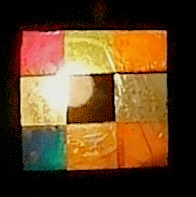
\includegraphics[width=0.75\textwidth]{figures/mica.jpg}
    \caption{Mica plate photo.}
    %\label{fig:}
\end{figure}

    
\end{minipage}

\phantom{42}

The rotation is observed by period $\pi/4$, as expected, with the coincidence of the main directions with the permitted areas of the oscillations of polaroids.